\subsection{What Is The Cumulative Haltiwanger Cross Contribution For Each Sector? \label{sec: veil}}

For each sector, I sum the cross contribution over each year of the `payroll labour share' sample
\begin{equation*}
    \underbrace{\sum_{t=1}^{T}\Delta\omega_{jt}\Delta\lambda_{jt}}_\text{Haltiwanger: Cross} 
\end{equation*}
Figure \ref{fig:veil} shows the cumulative Haltiwanger cross contribution is negative for virtually every sector. The reason is that, holding labour income $WL_{it}^{p}$ constant, changes in value-added $VA_{it}$ generate opposite movements in a sector's weight and labour share: $\Delta\omega_{it} > 0 \implies \Delta\lambda_{it} < 0$.

\begin{figure}[h]
  \centering
  \caption{\normalsize Size of cumulative cross contribution for each sector}
  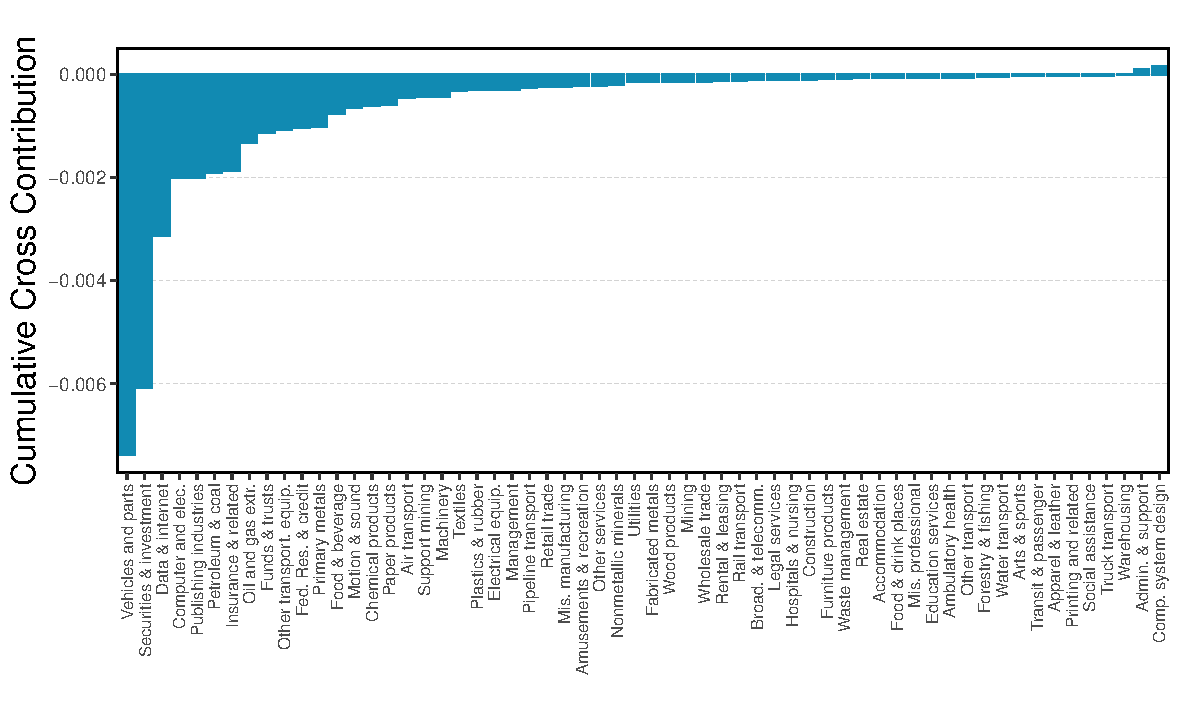
\includegraphics[width=14cm]{Decomposition/elsby_veil_total.pdf}
\begin{minipage}{\linewidth}
\captionsetup{justification=raggedright,singlelinecheck=false}
    \caption*{\textit{Notes}: Each bar indicates the cumulative sum of each sector's Haltiwanger cross contribution
  \begin{equation*}
    \underbrace{\sum_{t=1}^{T}\Delta\omega_{jt}\Delta\lambda_{jt}}_\text{Haltiwanger: Cross} 
  \end{equation*} \\
    \textit{Source}: BEA, \citet{elsbyDeclineLaborShare2013a} replication package, and author's calculations.}
\end{minipage}
  \label{fig:veil}
\end{figure}